\chapter{Zanka \texttt{while}}

\section{Kaj so zanke?}

Z uporabo stavka \texttt{if} lahko torej izbrane stavke izvedemo samo v primeru, ko je nek pogoj izpolnjen. Včasih pa bi želeli izbrane stavke izvajati vse \textbf{dokler} \angl{while} je nek pogoj izpolnjen. Slednje omogočajo \textbf{zanke}. V sledečem poglavju si bomo podrobneje pogledali zanko \texttt{while}. Razliko med izvedbo pogojnega stavka \texttt{if} in zanko \texttt{while} prikazuje slika \ref{img:while_vs_if}.

\begin{figure}
    \centering
    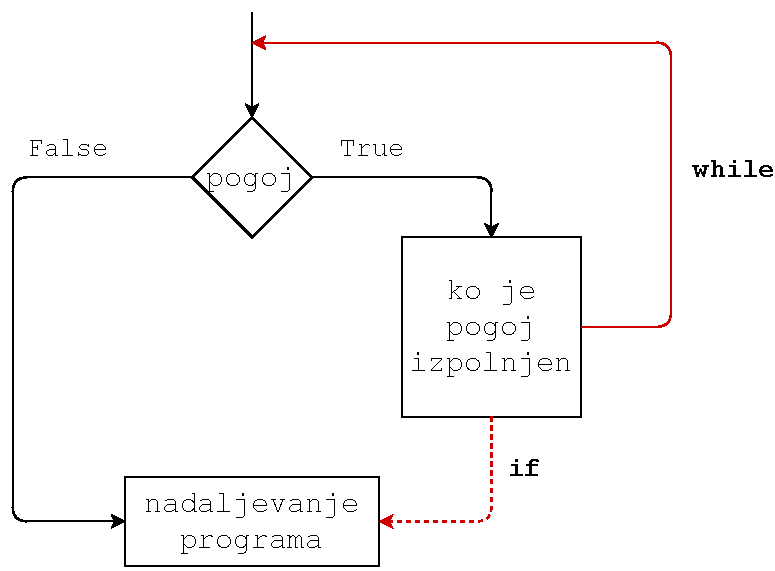
\includegraphics[width=0.5\linewidth]{img/while_vs_if.pdf}
    \caption{Razlika med izvedbo pogojnega stavka \texttt{if} (črtkana linija rdeče barve) in zanko \texttt{while} (polna linija rdeče barve). }
    \label{img:while_vs_if}
\end{figure}

\section{Zanka \texttt{while}}

Po izvedbi pogojnega dela stavka \texttt{if} se izvajanje programa nadaljuje v delu, ki sledi pogojnim stavkom. Po drugi strani se po izvedbi pogojnega dela zanke \texttt{while}, recimo tem stavkom raje \emph{telo zanke}, izpolnjenost pogoja v \emph{glavi zanke} ponovno preverja. Telo (vsebina) zanke se bo torej izvajalo vse dokler bo pogoj izpolnjen. Zanko \texttt{while} lahko zapišemo takole:
\begin{lstlisting}[language=Python]
while pogoj: # glava zanke
    # telo zanke
    ...
# nadaljevanje programa
...
\end{lstlisting}
Zapis zanke \texttt{while} je torej zelo podoben zapisu stavka \texttt{if}. Glavi zanke sledi telo zanke oziroma njena vsebina, ki se izvaja vse dokler je pogoj izpolnjen. Enemu obhodu zanke pravimo tudi \texttt{iteracija} zanke. Pogoje za izvedbo nove iteracije zanke lahko zapisujemo na popolnoma enak način kot pri stavku \texttt{if}. Prav tako kot pri stavku \texttt{if} vsebino zanke definiramo tako, da stavke znotraj telesa zanke zamikamo. Izvajanje zanke \texttt{while} ponazarja diagram poteka na sliki \ref{img:while1}.

\begin{figure}
    \centering
    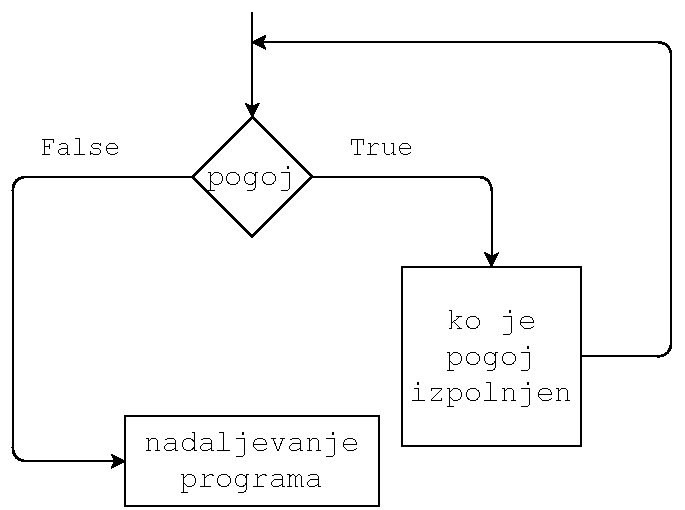
\includegraphics[width=0.5\linewidth]{img/while1.pdf}
    \caption{Potek izvajanja zanke \texttt{while}.}
    \label{img:while1}
\end{figure}

Zanke torej lahko uporabljamo takrat, ko želimo nekaj ponavljati dokler je določen pogoj izpolnjen. Npr., dokler uporabnik ne poda veljavnega vnosa, dokler ni števec dosegel določene vrednosti ali dokler sta števili različni. Končno lahko rešimo program, ki išče največji skupni delitelj dveh števil.
\begin{zgled}
Napiši program, ki od uporabnika prebere dve celi števili in poišče največji skupni delitelj teh dveh števil z uporabo Evklidovega algoritma.
\end{zgled}
\begin{resitev}
Program bo manjše število odšteval od večjega, dokler sta števili različni. Uporabili bomo torej zanko \texttt{while} (dokler sta števili različni).  Znotraj zanke bomo uporabili še stavek \texttt{if}, s pomočjo katerega bomo ugotovili, katero število je manjše. 
\begin{lstlisting}[language=Python,numbers=left]
st1 = int(input("Vnesi prvo stevilo: "))
st2 = int(input("Vnesi drugo stevilo: "))

while st1 != st2: # dokler sta stevili razlicni
    if st1 < st2: #drugo stevilo je vecje
        st2 = st2 - st1
    else: # prvo stevilo je veje
        st1 = st1 - st2

# konec vsebine zanke 
print(st1) # stevili sta tu enaki, zato je vseeno katero izpisem
\end{lstlisting}
Opomba: vsebina stavka \texttt{if} je zamaknjena dvakrat, saj je zapisana tako znotraj stavka \texttt{if} kot tudi znotraj zanke \texttt{while}!
\end{resitev}

\section{Štetje z zanko \texttt{while}}

Zanko \texttt{while} bi lahko uporabili tudi za štetje. Za ta namen je sicer boljša zanka \texttt{for}, do katere pridemo kasneje. Poglejmo si zgled.
\begin{zgled}
Napiši program, ki šteje od 0 do števila, ki ga je vnesel uporabnik. Vsa števila naj program tudi izpiše
\end{zgled}
\begin{resitev}
Število, do katerega smo prešteli, si bomo morali nekam zabeležiti, npr. v spremeneljivko z imenom \texttt{i}. Šteti bomo glede na navodila začeli s številom 0. Torej bomo spremenljivko \texttt{i} na začetku postavili na 0. Končali bomo s številom, ki ga je vnesel uporabnik, recimo \texttt{n}. Pogoj za štetje naprej bo torej \texttt{i <= n}. Znotraj zanke \texttt{while} bomo trenutno število (\texttt{i}) izpisali, poleg tega moramo pa trenutno število tudi povečati, saj bo sicer pogoj za vedno izpolnjen. 
\begin{lstlisting}[language=Python,numbers=left]
n = int(input("Vpisi stevilo do katerega zelis steti: "))
i = 0 # stevec s katerim bomo steli
while i <= n: # smo ze presteli?
    print(i)
    i = i + 1 # povecanje stevca za 1
\end{lstlisting}
\end{resitev}

\section{Stavek \texttt{+=}}
Znotraj zanke smo števec povečali za 1 z izvedbo prireditve
\begin{lstlisting}[language=Python]
i = i + 1 # povecanje stevca za 1
\end{lstlisting}
\texttt{i = i + 1}. Ker je tak način povečevanja vrednosti zelo pogost, v jeziku Python obstaja bližnjica
\begin{lstlisting}[language=Python]
i += 1 # povecanje stevca za 1
\end{lstlisting}
Bistvo zgornjega stavka je, da izvedemo aritmetično operacijo seštevanja in rezultat priredimo spremenljivki, nad katero smo operacijo izvedli. Na podoben način lahko operator prirejanja \texttt{=} kombiniramo z drugimi aritmetičnimi operatorji in števili:
\begin{lstlisting}[language=Python]
>>> x = 10
>>> x += 1 # povecaj za 1
>>> x
11
>>> x -= 2 # zmanjsaj za 2
>>> x
9
>>> x *= 5 # pomnozi s 5
>>> x
45
>>> x /= 9 # deli z 9
>>> x
5.0
>>> x **= 2 # potenciraj na 2
>>> x
25.0
\end{lstlisting}

\section{Mrtva zanka}

Kaj pa bi se zgodilo, če bi števec v prejšnjem zgledu znotraj zanke pozabili povečati? Spremenljivka \texttt{i} (oziroma števec) bi ostala na vrednosti 0 tudi po izvedbi zanke, kar pomeni, da bi bil pogoj za vedno izpolnjen (\texttt{True}). Kdaj bi se taka zanka končala? Ker je pogoj vedno resničen, se taka zanka nikoli ne konča in tak program je potrebno končati na silo (v okolju Python je temu namenjena kombinacija tipk \texttt{ctrl + c}). Na take stvari moramo torej pri programiranju z zanko \texttt{while} paziti. Zanki, ki se nikoli ne konča pravimo \emph{mrtva zanka} \angl{deadlock}.

\section{Stavek \texttt{break}}
Zanko pa lahko prekinemo tudi drugače kot z neizpolnjenostjo pogoja v glavi zanke. Uporabimo lahko namreč stavek \texttt{break}, ki prekine izvajanje zanke brez preverjanja pogoja v glavi zanke. Primer uporabe stavka \texttt{break} ponazarja spodnja koda
\begin{lstlisting}[language=Python]
while pogoj:
    # telo zanke
    ...
    if dodaten_pogoj: 
        break # prekine izvajanje zanke
# nadaljevanje programa
...
\end{lstlisting}
Izvedbo primera prikazuje slika \ref{img:while2}. 
\begin{figure}
    \centering
    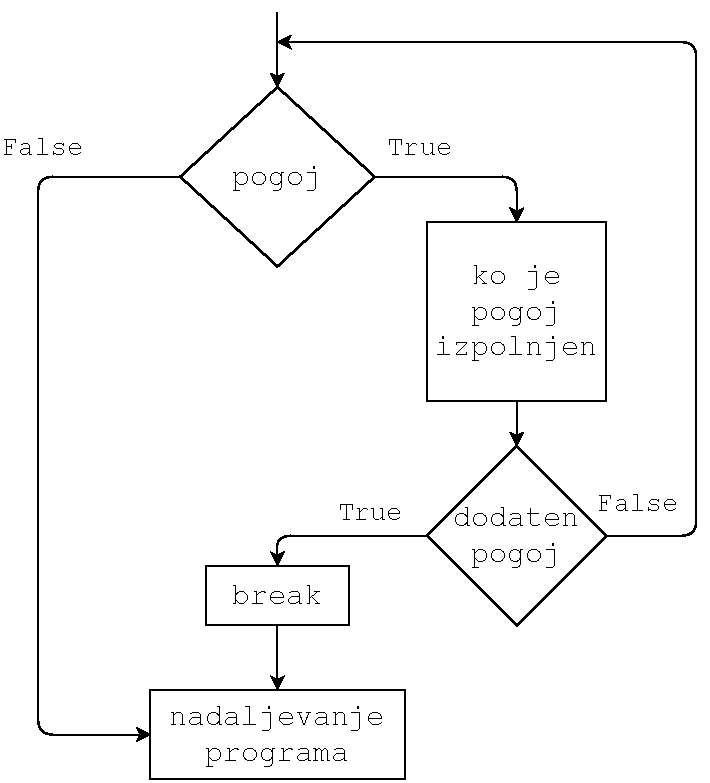
\includegraphics[width=0.5\linewidth]{img/while2.pdf}
    \caption{Primer uporabe stavka \texttt{break} znotraj zanke \texttt{while}.}
    \label{img:while2}
\end{figure}

Stavek \texttt{break} ponavadi uporabljamo v kombinaciji z dodatnim pogojem. V primeru, da je slednji izpolnjen. se izvajanje zanke prekine predčasno. Poglejmo si še en zgled, na katerem bomo potrenirali uporabo stavka \texttt{break}. 

\begin{zgled}
Napiši program, ki od uporabnika prebere dve celi števili in izpiše, če sta števili tuji. Števili sta tuji, če nimata nobenega skupnega delitelja, ki je večji od 1.
\end{zgled}
\begin{resitev}
Nalogo bi lahko rešili tako, da bi poiskali največji skupni delitelj podanih števil (naj bosta to števili \texttt{st1} in \texttt{st2})in pogledali, če je ta večji od 1. Tokrat se bomo rešitve lotili na malo drugačen način. Preverili bomo, če med kandidati za skupne delitelji obstaja kakšno število, ki deli obe števili, pri čemer bodo kandidati v razponu od števila 2 do manjšega števila, torej do vrednosti \texttt{min(st1, st2)}. V primeru, da med kandidati najdemo eno število, ki deli obe podani števili (ostanek po deljenju posameznega števila s kandidatom je enak 0 (\texttt{st \% kandidat == 0}), lahko takoj izpišemo, da števili nista tuji.
\begin{lstlisting}[language=Python,numbers=left]
st1 = int(input("Vnesi prvo stevilo: "))
st2 = int(input("Vnesi drugo stevilo: "))

delitelj = 2 # zacetna vrednost kandidata

while delitelj <= min(st1, st2): # kandidat gre do manjsega
    # ali kandidat deli obe stevili?
    if st1 % delitelj == 0 and st2 % delitelj == 0:
        print("Stevili nista tuji")
    delitelj += 1
\end{lstlisting}
Rešitev je še nepopolna, saj izpis poda samo v primeru, ko števili nista tuji. Kako bi lahko program dopolnili, tako da bi izpis podal tudi v primeru, ko sta števili tuji. Tak izpis lahko podamo samo v primeru, ko smo pregledali vse kandidate in nismo našli nobenega, ki deli obe števili. Pomagamo si lahko s pomožno spremenljivko tipa \texttt{bool}, v katero bomo shranili informacijo o tem, ali smo že našli kašnega delitelja. Pri tem bomo na začetku predpostavljali, da delitelja ni. Če ga bomo našli, bomo predpostavko popravili. Na koncu bomo preverili, če smo kakšnega delitelja našli. Če bo odgovor ne, bomo izpisali, da sta si števili tuji.
\begin{lstlisting}[language=Python,numbers=left]
st1 = int(input("Vnesi prvo stevilo: "))
st2 = int(input("Vnesi drugo stevilo: "))

delitelj = 2 # zacetna vrednost kandidata
# predspostavljamo, da skupnega delitelja se nismo nasli:
nasli = False 

while delitelj <= min(st1, st2): # kandidat gre do manjsega
    # ali kandidat deli obe stevili?
    if st1 % delitelj == 0 and st2 % delitelj == 0:
        print("Stevili nista tuji")
        nasli = True # popravimo predpostavko
    delitelj += 1

# ce do tu skupnega delitelja nismo nasli, potem ga ni        
if nasli == False: 
    print("Stevili sta tuji")
\end{lstlisting}
Program sicer deluje pravilno, je pa njegov izpis moteč, v primeru, da najdemo več skupnih deliteljev dveh števil. Vsakič, ko najdemo skupnega delitelja, namreč izpišemo, da smo ga našli
Poleg tega bi lahko izvajanje zanke \texttt{while} prekinili takoj, ko smo našli enega skupnega delitelja, saj je to zadosten pogoj, da si števili nista tuji. Uporabimo lahko torej stavek \texttt{break}. Končna rešitev bo sledeča.
\begin{lstlisting}[language=Python,numbers=left]
st1 = int(input("Vnesi prvo stevilo: "))
st2 = int(input("Vnesi drugo stevilo: "))

delitelj = 2 # zacetna vrednost kandidata
# predspostavljamo, da skupnega delitelja se nismo nasli:
nasli = False 

while delitelj <= min(st1, st2): # kandidat gre do manjsega
    # ali kandidat deli obe stevili?
    if st1 % delitelj == 0 and st2 % delitelj == 0:
        print("Stevili nista tuji")
        nasli = True # popravimo predpostavko
        break # lahko prenehamo z iskanjem
    delitelj += 1 

# ce do tu skupnega delitelja nismo nasli, potem ga ni        
if nasli == False: 
    print("Stevili sta tuji")
\end{lstlisting}
\end{resitev}

\section{Veja \texttt{else}}
Ena izmed posebnosti jezika Python je tudi to, da lahko vejo \texttt{else} uporabljamo tudi v kombinaciji z zanko \texttt{while}. Takole:
\begin{lstlisting}[language=Python]
while pogoj:
    # telo zanke
    ...
else:
    # ko pogoj ni vec izpolnjen
    ...
# nadaljevanje programa
...
\end{lstlisting}
Veja \texttt{else} se torej izvede, ko pogoj ni več izpolnjen. Vprašanje pa je ali se veja \texttt{else} izvede vsakič, ko se izvajanje zanke zaključi? Kakšna je razlika med stavki, ki sledijo zanki \texttt{while}, in stavki znotraj veje \texttt{else} zanke \texttt{while}? 

Do bistvene razlike med vejo \texttt{else} in običajnimi stavki, ki sledijo zanki \texttt{while}, pride, kadar zanko prekinemo s stavkom \texttt{break}. V tem primeru namreč skočimo iz zanke, s čimer preskočimo tudi njeno \texttt{else} vejo. Slednja se izvede samo v primeru, ko smo zanko prekinili po \emph{običajni} poti, tj. z neizpolnjenostjo pogoja v glavi zanke.  
\begin{lstlisting}[language=Python]
while pogoj:
    # telo zanke
    ...
    if dodaten_pogoj:
        break # prekini izvajanje zanke
else: # samo v primeru, ko zanka ni bila prekinjena z break
    # ko pogoj ni vec izpolnjen
    ...
# nadaljevanje programa
...
\end{lstlisting}
Delovanje zgornjega programa ponazarja slika \ref{img:while3}.
\begin{figure}
    \centering
    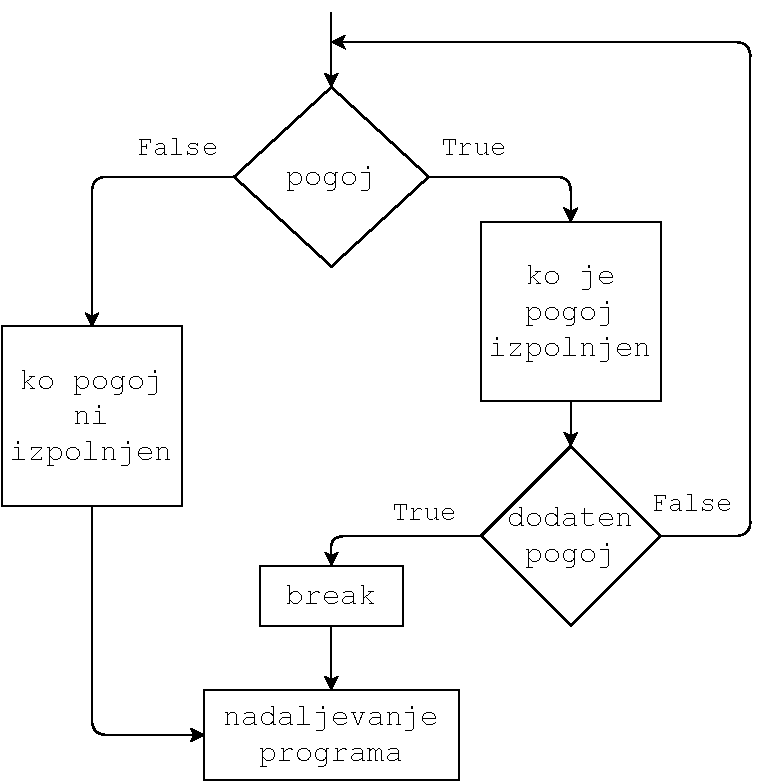
\includegraphics[width=0.5\linewidth]{img/while3.pdf}
    \caption{Primer uporabe stavka \texttt{break} v kombinaciji z vejo \texttt{else} za zanko \texttt{while}.}
    \label{img:while3}
\end{figure}
Določene stavke lahko po zaključku zanke \texttt{while} izvedemo samo v primeru, ko zanka ni bila prekinjena s stavkom \texttt{break}. Povadimo na prejšnjem zgledu še to.

\begin{zgled}
Napiši program, ki od uporabnika prebere dve celi števili in izpiše, če sta števili tuji. Števili sta tuji, če nimata nobenega skupnega delitelja, ki je večji od 1.
\end{zgled}
\begin{resitev}
Del programa, kjer izpisujemo, da si števili nista tuji, bo ostal bolj ali manj nespremenjen. Skrajšamo pa lahko tiste dela programa, ki jih potrebujemo za izpis, da sta si števili tuji. Števili sta si tuji, ko nismo našli nobenega skupnega delitelja. To se zgodi takrat, ko se je zanka \texttt{while} \emph{odvrtela} do konca in nismo našli nobenega skupnega delitelja, torej je posledično nismo prekinili s stavkom \texttt{break}. Če zanko \texttt{while} dopolnimo z \texttt{else} vejo, se bo ta izvedla natanko takrat, ko zanka ni bila prekinjena s stavkom \texttt{break}, torej takrat, ko nismo našli nobenega skupnega delitelja. Znotraj veje \texttt{else} lahko torej zapišemo, da sta si števili tuji. Na tak način se lahko znebimo spremenljivke \texttt{nasli} in naredimo program krajši in bistveno bolj pregleden.
\begin{lstlisting}[language=Python,numbers=left]
st1 = int(input("Vnesi prvo stevilo: "))
st2 = int(input("Vnesi drugo stevilo: "))

delitelj = 2 # zacetna vrednost kandidata

while delitelj <= min(st1, st2): # kandidat gre do manjsega
    # ali kandidat deli obe stevili?
    if st1 % delitelj == 0 and st2 % delitelj == 0:
        print("Stevili nista tuji")
        break # lahko prenehamo z iskanjem
    delitelj += 1 
else: # ali se je zanka odvrtela do konca
    # zanke nismo prekinili s stavkom break
    print("Stevili sta tuji")
\end{lstlisting}
\end{resitev}